\section{事件概率的计算}
\label{sec:cprob-computing}

有了式~\eqref{eq:cprob-classical}，计算概率就是数两个集合。真正的困难在于数对：样本空间要选得等可能，事件要在同一个样本空间里数，补、并、交这些组合事件要用合适的方式拆开。本节先整理抽样问题中常用的计数公式，再分别处理补事件、并事件和交事件。

\paragraph{四种抽样方式}
从$n$个可区分的对象中取$k$次，按“是否放回”和“是否记录次序”可以分成四种情形。各自的结果个数在\BookChapterRef{chap:counting}{卷一第2章“计数”}中已经得到，记$P(n,k)=n(n-1)\cdots(n-k+1)$为排列数，$\binom nk$为组合数。表~\ref{tab:cprob-sampling}把它们放在一起，并标出每种记录下的结果是否同样可能。

\begin{BookInlineTable}
  \centering
  \caption{从$n$个对象中取$k$次的四种记录方式}
  \label{tab:cprob-sampling}
  \begin{tabular}{llll}
    \toprule
    记录方式 & 结果的形式 & 结果个数 & 是否等可能 \\
    \midrule
    不放回、有序 & 无重复的$k$元有序组 & $P(n,k)$ & 是 \\
    不放回、无序 & $k$元子集 & $\binom nk$ & 是 \\
    放回、有序 & 可重复的$k$元有序组 & $n^{k}$ & 是 \\
    放回、无序 & 可重复的$k$元组合 & $\binom{n+k-1}{k}$ & 否 \\
    \bottomrule
  \end{tabular}
\end{BookInlineTable}

前三种的等可能性来自同一个物理假设：每次取样时，剩下的各对象被取到的机会相同。有序记录直接继承这一假设。不放回的无序记录中，每个$k$元子集恰好由$k!$个有序组忘去次序得到，各子集合并的有序组个数相同，所以仍等可能。放回的无序记录则不然：取两次时，组合$\{1,1\}$只来自有序组$(1,1)$，组合$\{1,2\}$却来自$(1,2)$和$(2,1)$两个。这一行不能直接用于计数比，第~\ref{sec:cprob-scope}节再回到它。

\paragraph{分子与分母同一口径}
在摸球问题中计算“两个都是黑球”的概率。用有序记录，分母是$P(5,2)=20$，分子是从$3$个黑球中有序地取$2$个，$P(3,2)=6$；用无序记录，分母是$\binom52=10$，分子是$\binom32=3$。两种算法给出
\[
 \frac{P(3,2)}{P(5,2)}=\frac{6}{20}=\frac{3}{10},\qquad
 \frac{\binom32}{\binom52}=\frac{3}{10}.
\]
结果一致。若分子用无序的$3$、分母用有序的$20$，就得到$3/20$，这个数不是任何事件的概率。

两种口径给出同一结果并非巧合。“两个都是黑球”只关心摸到了哪些球，不关心先后。对这样的事件，每个满足条件的子集恰好对应$k!$个满足条件的有序组，分子和分母同乘以$k!$，比值不变。这个论证也说明了口径一致的含义：分子和分母必须是同一个样本空间中的计数。

事件“恰好一个黑球”同样只与内容有关。无序记录中它有$3\times2=6$个子集，有序记录中有$3\times2\times2=12$个有序对，概率都是$3/5$。事件“第一个是黑球”则与次序有关，只能在有序记录中数：第一个位置有$3$种，第二个位置从剩下$4$个中任取，共$12$个，概率也是$3/5$。

\paragraph{一副牌中的组合计数}
从一副$52$张的扑克牌中随机抽$3$张，不放回。每个$3$张的子集同样可能。事件“$3$张都是红桃”要求$3$张全部取自$13$张红桃，所以
\[
 \mathbb{P}(\text{三张都是红桃})=\frac{\binom{13}{3}}{\binom{52}{3}}
 =\frac{286}{22100}=\frac{11}{850}\approx0.0129.
\]
第~\ref{sec:cprob-conditional}节会用逐张抽取的方式重新得到这个数。

事件较复杂时，常把满足条件的结果拆成几步来构造，再用乘法规则计数。这时要检查两件事：每一步的选择合起来恰好得到事件中的一个结果，事件中的每个结果也只由一种选择方式得到。以抽$5$张牌“恰好一对”为例，它要求有两张点数相同，其余三张的点数互不相同，也都不同于这一对。

按下面的步骤构造：先选成对的点数，有$13$种；再选这一对的两种花色，有$\binom42=6$种；再从其余$12$个点数中选出三个单张的点数，有$\binom{12}{3}=220$种；最后给三个单张各选一种花色，有$4^{3}=64$种。每手“恰好一对”的牌由唯一一组选择得到，所以
\[
 \mathbb{P}(\text{恰好一对})=\frac{13\times6\times220\times64}{\binom{52}{5}}
 =\frac{1098240}{2598960}\approx0.4226.
\]

一种常见的错误算法是：选好一对之后，从剩下的$48$张牌中任取$3$张，得到$13\times6\times\binom{48}{3}$。这样取出的三张可能又凑成一对，或与已选的一对同点数，于是两对、三条等牌型也被算了进去，而且一手两对的牌按“哪一对先选”会被数两次。另一种错误是把三个单张的点数按$12\times11\times10$有序地选，每手牌被重复数了$3!$次。两种错误都破坏了“恰好一个结果对应一种选择”。

\paragraph{补事件}
“至少一个”“不全相同”这类事件往往由许多情形组成，直接数很麻烦，它的反面却只有一种或少数几种情形。下面的公式把概率转到补事件上。

\begin{theorem}[补事件与包含关系]
\label{thm:cprob-complement}
在古典概率模型中，对任意事件$A$，
\begin{equation}
 \mathbb{P}(A^{\mathrm{c}})=1-\mathbb{P}(A).
 \label{eq:cprob-complement}
\end{equation}
若$A\subseteq B$，则
\begin{equation}
 \mathbb{P}(B\setminus A)=\mathbb{P}(B)-\mathbb{P}(A),\qquad
 \mathbb{P}(A)\leq\mathbb{P}(B)\leq1.
 \label{eq:cprob-monotone}
\end{equation}
特别地，$\mathbb{P}(\varnothing)=0$。
\end{theorem}

\begin{proof}
若$A\subseteq B$，则$B$是互斥的$A$与$B\setminus A$之并。由互斥可加性~\eqref{eq:cprob-additive}，
\[
 \mathbb{P}(B)=\mathbb{P}(A)+\mathbb{P}(B\setminus A).
\]
移项得到式~\eqref{eq:cprob-monotone}的等式；由非负性~\eqref{eq:cprob-nonneg}，$\mathbb{P}(B\setminus A)\geq0$，所以$\mathbb{P}(A)\leq\mathbb{P}(B)$。取$B=\Omega$，用归一性~\eqref{eq:cprob-normalized}，就得到式~\eqref{eq:cprob-complement}与$\mathbb{P}(B)\leq1$。再取$A=\Omega$，得到$\mathbb{P}(\varnothing)=1-1=0$。
\end{proof}

证明只用了三条基本性质，没有再回到计数。这一点后面很重要：凡是满足这三条性质的概率分配，补事件公式都成立。

\paragraph{生日问题}
一个班有$n$个人，至少两人同一天生日的概率是多少？作模型假设：一年按$365$天计，每人的生日在$365$天中等可能，各人之间互不影响。依次写下$n$个人的生日，结果是可重复的有序组，样本空间有$365^{n}$个等可能的点。

“至少两人同一天”包含两人相同、三人相同、两对分别相同等许多情形；它的补事件“$n$个生日两两不同”只有一种情形，正是不放回的有序取法，共$P(365,n)$个。由式~\eqref{eq:cprob-complement}，
\begin{equation}
 \mathbb{P}(\text{至少两人同一天生日})
 =1-\frac{P(365,n)}{365^{n}}
 =1-\prod_{i=0}^{n-1}\Bigl(1-\frac{i}{365}\Bigr).
 \label{eq:cprob-birthday}
\end{equation}

代入$n=23$，乘积约为$0.4927$，所求概率约为$0.5073$，已经超过一半；$n=50$时约为$0.970$。图~\ref{fig:cprob-birthday}画出了它随$n$的变化。这个结果常常出人意料，原因在于要比较的是人与人之间的配对，$23$个人之间有$\binom{23}{2}=253$对，每一对都可能撞上。

\begin{BookInlineFigure}
  \centering
  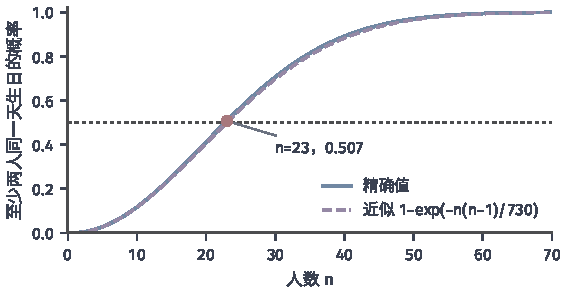
\includegraphics[width=96mm]{figures/07-probability/01-elementary-probability/matplotlib/cprob-birthday/figure.pdf}
  \caption{生日问题。蓝线是式~\eqref{eq:cprob-birthday}的精确值，紫色虚线是近似$1-\exp(-n(n-1)/730)$，黑色点线是$1/2$；红点标出$n=23$时的$0.507$。}
  \label{fig:cprob-birthday}
\end{BookInlineFigure}

配对的说法可以变成一个不等式。由$1-x\leq\mathrm{e}^{-x}$对所有实数$x$成立，乘积中每个因子都不超过$\mathrm{e}^{-i/365}$；$n\leq365$时各因子非负，不等式可以逐项相乘，于是
\[
 \prod_{i=0}^{n-1}\Bigl(1-\frac{i}{365}\Bigr)
 \leq\exp\Bigl(-\sum_{i=0}^{n-1}\frac{i}{365}\Bigr)
 =\exp\Bigl(-\frac{n(n-1)}{730}\Bigr).
\]
指数中的$n(n-1)/2$正是配对数。$n=23$时右端为$\mathrm{e}^{-506/730}\approx0.499998$，略小于$1/2$，所以不需要计算乘积，就知道所求概率大于$1/2$。图中紫色虚线与蓝线几乎重合，说明$i/365$较小时这个上界也很接近真实值。

\paragraph{并事件}
两个事件的并，直接相加会出错：$\lvert A\rvert+\lvert B\rvert$把$A\cap B$中的结果数了两次。减去重复的部分，就是计数的容斥原理在概率中的形式。

\begin{theorem}[加法公式]
\label{thm:cprob-addition}
在古典概率模型中，对任意事件$A,B$，
\begin{equation}
 \mathbb{P}(A\cup B)=\mathbb{P}(A)+\mathbb{P}(B)-\mathbb{P}(A\cap B).
 \label{eq:cprob-addition}
\end{equation}
对三个事件$A,B,C$，
\begin{equation}
 \begin{aligned}
 \mathbb{P}(A\cup B\cup C)
 &=\mathbb{P}(A)+\mathbb{P}(B)+\mathbb{P}(C)\\
 &\quad-\mathbb{P}(A\cap B)-\mathbb{P}(A\cap C)-\mathbb{P}(B\cap C)\\
 &\quad+\mathbb{P}(A\cap B\cap C).
 \end{aligned}
 \label{eq:cprob-inclusion-exclusion}
\end{equation}
\end{theorem}

\begin{proof}
$A\cup B$可以拆成互斥的三块$A\setminus B$、$A\cap B$、$B\setminus A$；$A$是前两块之并，$B$是后两块之并。由互斥可加性~\eqref{eq:cprob-additive}，
\[
 \begin{aligned}
 \mathbb{P}(A\cup B)&=\mathbb{P}(A\setminus B)+\mathbb{P}(A\cap B)+\mathbb{P}(B\setminus A),\\
 \mathbb{P}(A)+\mathbb{P}(B)&=\mathbb{P}(A\setminus B)+2\,\mathbb{P}(A\cap B)+\mathbb{P}(B\setminus A).
 \end{aligned}
\]
两式相减即得式~\eqref{eq:cprob-addition}。

对三个事件，把$B\cup C$看成一个事件，先用一次式~\eqref{eq:cprob-addition}：
\[
 \mathbb{P}(A\cup B\cup C)=\mathbb{P}(A)+\mathbb{P}(B\cup C)-\mathbb{P}\bigl((A\cap B)\cup(A\cap C)\bigr).
\]
再对$\mathbb{P}(B\cup C)$和最后一项各用一次式~\eqref{eq:cprob-addition}，注意$(A\cap B)\cap(A\cap C)=A\cap B\cap C$，整理即得式~\eqref{eq:cprob-inclusion-exclusion}。
\end{proof}

对$m$个事件，同样的公式在交替加减所有$k$个事件之交的概率后成立，它是有限容斥原理两边同除以$\lvert\Omega\rvert$的结果。丢掉式~\eqref{eq:cprob-addition}中非负的一项$\mathbb{P}(A\cap B)$，得到
\begin{equation}
 \mathbb{P}(A\cup B)\leq\mathbb{P}(A)+\mathbb{P}(B),
 \label{eq:cprob-union-bound}
\end{equation}
对事件个数归纳可推广到任意有限个事件，称为\term{联合界}（union bound）。它不要求事件之间有任何关系，常用来估计“至少一处出问题”的概率。

\paragraph{至少一个六点}
掷两枚骰子，求至少出现一个六点的概率。令$A$为“第一枚是六点”，$B$为“第二枚是六点”，所求事件是$A\cup B$。$A$与$B$各占$6$格，它们只在$(6,6)$这一格重叠，如图~\ref{fig:cprob-at-least-one-six}(a)所示。由式~\eqref{eq:cprob-addition}，
\[
 \mathbb{P}(A\cup B)=\frac{6}{36}+\frac{6}{36}-\frac{1}{36}=\frac{11}{36}.
\]

\begin{BookInlineFigure}
  \centering
  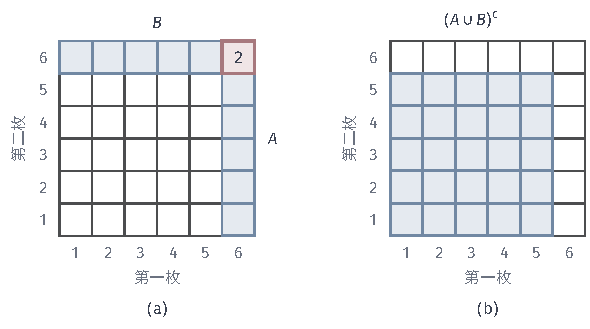
\includegraphics[width=100mm]{figures/07-probability/01-elementary-probability/tikz/cprob-at-least-one-six/figure.pdf}
  \caption{两枚骰子中至少一个六点。(a)浅蓝的一列是$A$（第一枚六点），浅蓝的一行是$B$（第二枚六点），红格$(6,6)$在$\lvert A\rvert+\lvert B\rvert$中被数了两次。(b)补事件“两枚都不是六点”是$5\times5$的方块。}
  \label{fig:cprob-at-least-one-six}
\end{BookInlineFigure}

用补事件计算更直接。由De Morgan律，$(A\cup B)^{\mathrm{c}}$就是$A^{\mathrm{c}}\cap B^{\mathrm{c}}$，即“两枚都不是六点”，即图~\ref{fig:cprob-at-least-one-six}(b)中$5\times5=25$个格子，所以概率是$1-25/36=11/36$，两种算法一致。

掷三枚骰子时两种方法的差别更明显。用式~\eqref{eq:cprob-inclusion-exclusion}，单个事件各占$36$个结果，两两之交各占$6$个，三者之交占$1$个，于是
\[
 \mathbb{P}(\text{至少一个六点})=\frac{3\times36-3\times6+1}{216}=\frac{91}{216}.
\]
用补事件，“三枚都不是六点”有$5^{3}=125$个结果，概率是$1-125/216=91/216$。补事件只需要一次计数，容斥原理需要逐层修正。

\paragraph{交事件}
交事件要求几个条件同时满足，一般要在样本空间中把两个条件一起数。在摸球问题的有序记录中，令$H_1$为“第一个是黑球”，$E$为“两个球颜色不同”。$H_1\cap E$就是“第一个黑、第二个白”，有$3\times2=6$个有序对，所以$\mathbb{P}(H_1\cap E)=6/20$。

此时$\mathbb{P}(H_1)=12/20$，$\mathbb{P}(E)=12/20$，二者相乘得$0.36$，并不等于$0.3$。交事件的概率一般不能由各自的概率相乘得到；什么时候可以相乘，是第~\ref{sec:cprob-independence}节的问题。

\paragraph{放回与不放回}
最后固定一个抽检问题，比较放回与不放回。一批$20$件产品中有$4$件次品，随机抽取$5$件检查。不放回时，每个$5$件子集等可能，“没有次品”要求$5$件都取自$16$件合格品：
\[
 \mathbb{P}_{\text{不放回}}(\text{没有次品})=\frac{\binom{16}{5}}{\binom{20}{5}}=\frac{4368}{15504}\approx0.2817.
\]
若改用不放回的有序记录，分子分母分别是$P(16,5)$和$P(20,5)$，比值不变。

放回时，每次都从全部$20$件中取，有序记录有$20^{5}$个等可能结果，其中每次都取到合格品的有$16^{5}$个：
\[
 \mathbb{P}_{\text{放回}}(\text{没有次品})=\Bigl(\frac{16}{20}\Bigr)^{5}=0.32768.
\]
放回时同一件合格品可以被反复抽到，合格品“用不完”，所以全是合格品的机会更大。

两种方式下“恰好一件次品”的计数方法不同。不放回时选$1$件次品、$4$件合格品，概率为
\[
 \frac{\binom41\binom{16}{4}}{\binom{20}{5}}=\frac{7280}{15504}\approx0.4696.
\]
放回时必须用有序记录：先选次品出现在哪一次，有$5$种；该次有$4$种取法，其余四次各有$16$种。于是概率为
\[
 \frac{5\times4\times16^{4}}{20^{5}}=0.4096.
\]
这里不能把放回的结果按无序组合来数，因为表~\ref{tab:cprob-sampling}最后一行的结果不等可能。

图~\ref{fig:cprob-replacement-compare}把“没有次品”的概率画成抽取件数$k$的函数。不放回的曲线始终低于放回的曲线，并在$k=17$时降到$0$：$17$件中至少有一件次品，因为合格品只有$16$件。$k$相对于$20$较小时两条曲线很接近，每次抽走一件对剩余构成的影响较小。

\begin{BookInlineFigure}
  \centering
  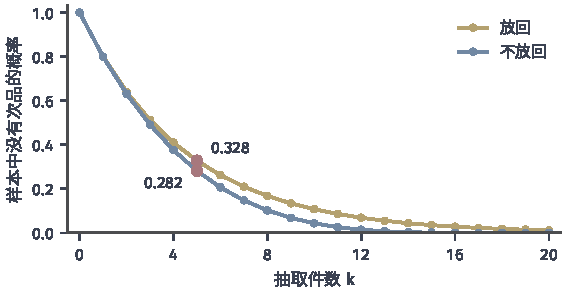
\includegraphics[width=96mm]{figures/07-probability/01-elementary-probability/matplotlib/cprob-replacement-compare/figure.pdf}
  \caption{$20$件中含$4$件次品时，抽取$k$件都是合格品的概率。蓝线是不放回抽样$\binom{16}{k}/\binom{20}{k}$，黄线是放回抽样$0.8^{k}$；红点标出正文中$k=5$的两个值。}
  \label{fig:cprob-replacement-compare}
\end{BookInlineFigure}
